\documentclass[11pt]{article}

\usepackage{graphicx}
\graphicspath{ {./assets/} }
\usepackage{tabulary}
\usepackage{booktabs, multirow} 
\usepackage{soul}
\usepackage[table]{xcolor}
\usepackage{changepage,threeparttable} 

\usepackage{geometry}
 \geometry{
 a4paper,
 left=34mm,
 top=27mm,
 right=20mm,
 }
 \usepackage[hidelinks
 ]{hyperref}
\sloppy
\author{Jonas Jacob Biermann}
\title{Der Reversible Kailum-Iod Akku}

\begin{document}
\maketitle
\tableofcontents

\newpage

\section{Aufgabe}
Untersuchen Sie die Reversibilität der chemischen Reaktion innerhalb eines Kalium-Iod-Akkumulators in Hinblick auf die Spannungskurve beim Entladevorgang.

\section{Vorbetrachtung}

\subsection{Funktionsweise Akkumulator}
Ein Akkumulator besteht aus einer negativen und einer positiven Elektrode, die in einer Elektrolytlösung getaucht sind. Während des Entladevorgangs fließen Elektronen von der negativen zur positiven Elektrode durch einen externen Stromkreislauf, während Ionen durch den Elektrolyten wandern, um die Ladung aufrechtzuerhalten. Beim Ladevorgang wird der Prozess umgekehrt, indem die Elektronen von der positiven zur negativen Elektrode fließen und die Ionen in die entgegengesetzte Richtung wandern, um die Energie in Form von chemischen Bindungen zwischen den Elektroden und dem Elektrolyten zu speichern. Die chemischen Prozesse, die in einem Akkumulator ablaufen, hängen von der Art des Akkumulators ab, wie zum Beispiel Blei-Säure-Akkumulatoren, Lithium-Ionen-Akkus oder Nickel-Metallhydrid-Akkus.

\subsection{Vorgänge an den Elektroden}
Wie bereits erwähnt, ist ein Akkumulator aus einer Kathode und aus einer Anode aufgebaut. Dabei läuft an der Kathode eine Reduktionsreaktion und bei der Anode eine Oxidationsreaktion ab. Dementsprechend werden an der Kathode Elektronen von den Ionen aufgenommen und an der Anode Elektroden von den Ionen abgegeben. Die Reaktionen funktionieren jeweils in beide Richtungen, was dann den Auf- beziehungsweise den Entladevorgang beschreibt.

\subsection{Reaktionsgleichungen}
Bei dem Experiment zum Kalium-Iod-Akku laufen folgende Vorgänge an den Elektroden ab:\\
1. An der Anode findet eine Oxidationsreaktion von Iodidionen zu Iod statt:
\begin{center}
    \begin{equation}
        2 I^{-} \rightleftharpoons I_{2} + 2 e^{-}
    \end{equation}
\end{center}

\noindent
2. An der Kathode findet eine Reaktion von Kaliumionen zu Kalium statt:
\begin{center}
    \begin{equation}
        K^{+} + e^{-} \rightleftharpoons K
    \end{equation}
\end{center}

\noindent
3. Dementsprechend lautet die vollständige Reaktionsgleichung:
\begin{center}
    \begin{equation}
        2 K^{+} + 2 I^{-} \rightleftharpoons 2 K + I_{2}
    \end{equation}
\end{center}

\subsection{Elektronegativität}
Die Elektronegativität ist eine Maßzahl für die Fähigkeit eines Atoms, Elektronen in einer chemischen Bindung zu sich zu ziehen. Sie beschreibt die relativen Kräfte, mit denen Atome in einer Bindung Elektronen anziehen und ist ein wichtiger Parameter in der Chemie. Die Elektronegativität wird in der Regel auf einer Skala angegeben, wobei das Element Fluor mit dem höchsten Wert von 4,0 als Referenz dient. Je höher die Elektronegativität eines Atoms, desto stärker zieht es Elektronen an und desto polarer ist die chemische Bindung.

\subsection{Elektrochemisches Standardpotential}
Das elektrochemische Standardpotential ist das Reduktionspotential einer Elektrode bei Standardbedingungen ($25^{\circ}C, 1 \:atm, 1 \:\frac{mol}{l}$). Es wird als Referenzpotential für die elektrochemische Spannungsreihe verwendet, um die relativen Redoxpotentiale anderer Elemente oder Verbindungen zu bestimmen.

\subsection{Elektrochemische Spannungsreihe}
Die elektrochemische Spannungsreihe ist eine Liste von Metallen und Halbmetallen, die nach ihrer Tendenz sortiert sind, Elektronen abzugeben und somit zu oxidieren. Die Spannungsreihe gibt an, welche Metalle stärker oxidiert werden können als andere. Die Spannungsreihe beruht auf der Beobachtung, dass in einem galvanischen Element, das aus zwei unterschiedlichen Metallen und einer Elektrolytlösung besteht, das Metall mit dem niedrigeren Potential oxidiert wird und Elektronen abgibt, während das Metall mit dem höheren Potential reduziert wird und Elektronen aufnimmt.
Das Standardpotential 0V bezieht sich auf das Reduktionspotential eines Wasserstoffions ($H^{+}$) bei Standardbedingungen ($25^{\circ}C, 1 \:atm, 1 \:\frac{mol}{l}$). Es wird als Referenzpotential für die elektrochemische Spannungsreihe verwendet, um die relativen Redoxpotentiale anderer Elemente oder Verbindungen zu bestimmen. Ein positives Redoxpotential bedeutet, dass die betreffende Substanz oxidierend wirkt, während ein negatives Redoxpotential auf eine reduzierende Wirkung hinweist.

\subsection{Elektrolyse}
Elektrolyse bezieht sich auf den Prozess der chemischen Zersetzung von Verbindungen durch die Anwendung einer elektrischen Energie. Es handelt sich um einen nicht-spontanen Prozess, bei dem elektrische Energie in chemische Energie umgewandelt wird. Die Elektrolyse findet in einer elektrolytischen Zelle statt, die aus einer Kathode (negativ geladene Elektrode), einer Anode (positiv geladene Elektrode) und einer Elektrolytlösung besteht. Beim Anlegen einer elektrischen Spannung an die Elektroden werden die Ionen in der Elektrolytlösung zur Kathode oder Anode gezogen, je nachdem ob es sich um Kationen oder Anionen handelt. An der Kathode findet die Reduktion statt, während an der Anode die Oxidation stattfindet. Dadurch können Verbindungen in ihre Bestandteile zersetzt werden oder auch neue Verbindungen gebildet werden. Die Elektrolyse hat zahlreiche Anwendungen, z.B. in der Gewinnung von Metallen oder der Herstellung von chemischen Produkten.

\subsection{Reversibilität einer chemischen Reaktion im Akku}
Die Reversibilität einer chemischen Reaktion im Akku bezieht sich auf die Fähigkeit einer elektrochemischen Zelle, eine chemische Reaktion in beide Richtungen durchzuführen, dh sowohl Ladung als auch Entladung zu ermöglichen. Eine reversible Reaktion im Akku ermöglicht es, dass die Elektroden und der Elektrolyt ihre ursprüngliche chemische Zusammensetzung wiedererlangen, wenn eine umgekehrte elektrische Spannung an die Zelle angelegt wird. Dies ist wichtig, um die Lebensdauer und die Leistungsfähigkeit des Akkus aufrechtzuerhalten.

\subsection{Hypothese}
Es wird davon ausgegangen, dass sich beim Aufladen der farblosen Kalium-Iod-Lösung die Lösung an einer der beiden Graphit-Elektroden gelblich verfärbt, da hier das gelbe Iod beim aufladen aus Iodid-Ionen gewonnen wird. Dementsprechend sollte umgekehrt die gelbe Farbe nach dem Entladen verschwinden. Außerdem wird eine Entladekurve, also die Spannung des Akkus beim Entladen, aufgenommen, wobei davon ausgegangen werden kann, dass diese invers exponentiell verlaufen wird. Außerdem sollte sich die Leistung des Kalium-Iod-Akkumulators nach mehreren Messungen etwas verschlechtern. 

\section{Geräte, Hilfsmittel und Chemikalien}
\begin{center}

    \begin{tabular}{ c|c|c } 
        Geräte & Hilfsmittel & Chemikalien \\ 
        \hline
        Stromquelle & Krokodilklammern & Kaliumiodid \\ 
        Multimeter & Kabel & destilliertes Wasser \\
        U-Rohr & Spatellöffel & Graphitelektroden \\
        Maßkolben & Stativklemme & - \\
        Waage & Stativ & - \\ 
       \end{tabular}

\end{center}
\noindent
Das Kaliumiodid (H372 und P314) ist die einzige Chemikalie mit H- und P-Sätzen.

\section{Skizze und Aufbau}
\begin{figure}[h!]
    \centering
    \caption{Skizze des Experiments}
    \label{fig:skizze}
    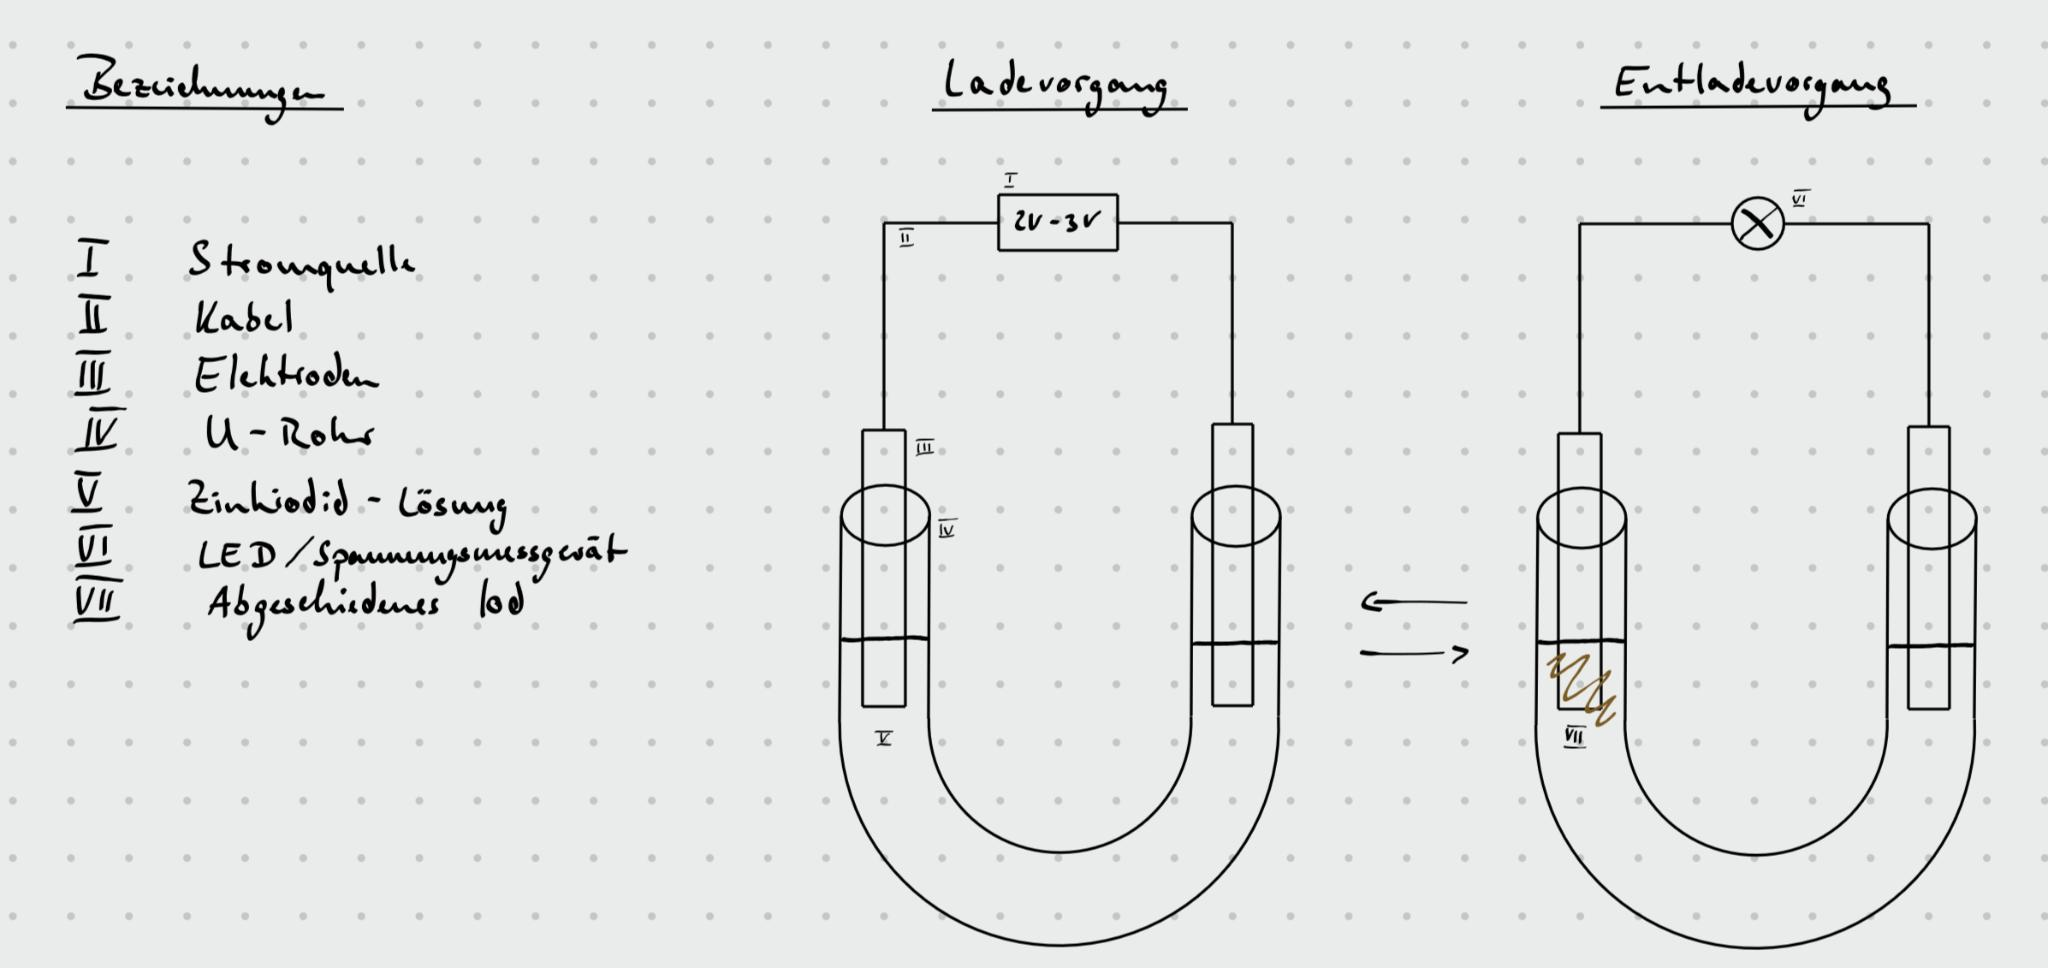
\includegraphics[scale=0.185]{figure.png}
\end{figure}
\begin{figure}[h!]
    \centering
    \caption{Aufbau des Experiments}
    \label{fig:aufbau}
    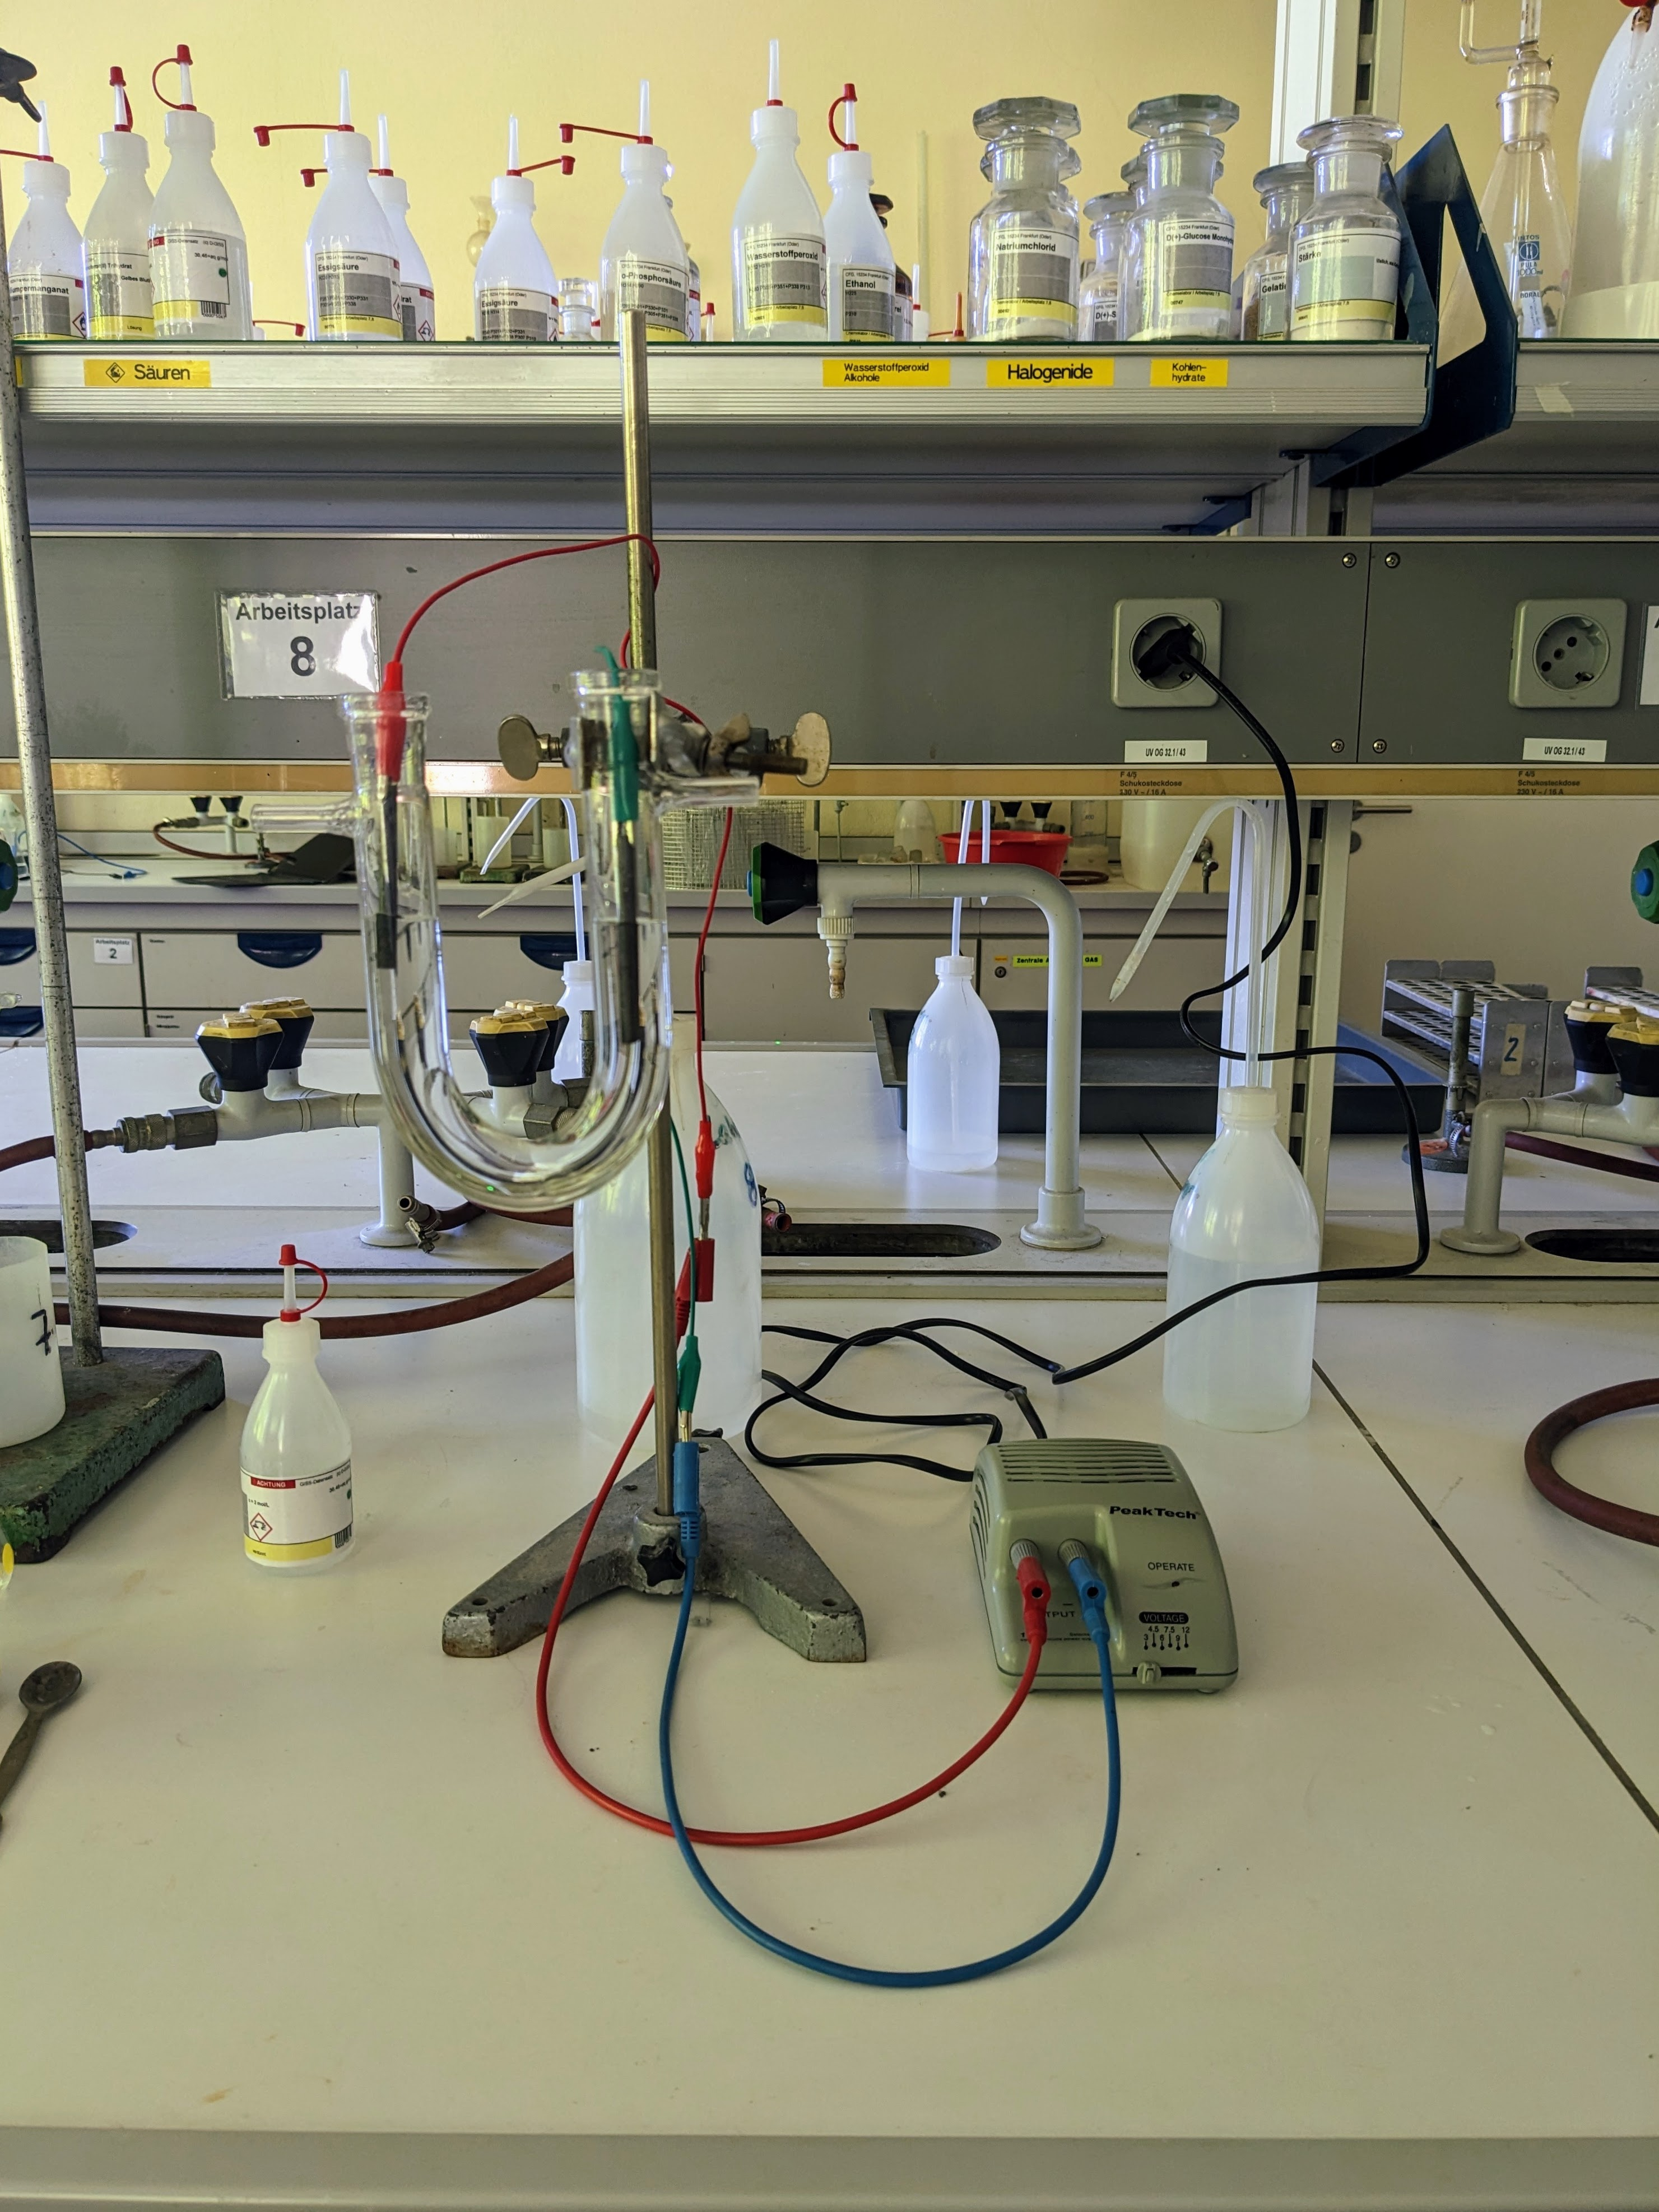
\includegraphics[scale=0.08]{aufbau.jpg}
\end{figure}

\section{Durchführung und Beobachtung}
Zunächst muss eine Kaliumiodid-Lösung hergestellt werden. Dazu werden $1.5\:g$ Kaliumiodid abgewogen und in einen $50\:mL$ Maßkolben, welcher mit destilliertem Wasser gefüllt ist, gegeben. Es konnte festgestellt werden, dass die Lösung farblost ist.\\
\newline
\noindent
Im Anschluss wird das U-Rohr mit Hilfe einer Stativklemme an einem Stativ befestigt und die Kaliumiodid-Lösung eingefüllt. Die Stormquelle wird an den Storm angeschlossenen, wobei sie ausgeschaltet bleibt, und die Elektroden werden mit Hilfe von Krokodilklammern und Kabeln mit der Stormquelle verkabelt.
\begin{center}
\begin{tabulary}{1\textwidth}{L|C|C}
     & Durchführung & Beobachtung\\
    \hline
    1. & Ausgangszustand & Farblose Lösung\\
    \hline
    2. & Stomquelle für 5 Minuten einschalten & Gelber Faden erkennbar an linker Elektrode, gelbliche Verfärbung der Lösung\\
    \hline
    3. & Zwischenzustand & Gelbe Lösung, gelber Faden an Elektrode bleibt\\
    \hline
    4.1 & Kabel umstecken von Stromquelle auf Multimeter & -\\
    \hline
    4.2 & alle $10\:s$ wird ein Wert aufgenommen & starker Abfall der Spannung, kaum farbliche Veränderung erkennbar\\
    \hline
    5. & nach 8.5 Minuten Widerholung Schritte 2 bis 4 & Lösung bleibt durchgängig Gelb, Spannung fällt bei Entladevorgang\\

\end{tabulary}
\end{center}
\noindent
Die gelbe Färbung an der Graphit-Elektrode wird in Abbildung \ref{fig:beobachtung} klar sichtbar.

\begin{figure}[h!]
    \centering
    \caption{Beobachtung Verfärbung Lösung}
    \label{fig:beobachtung}
    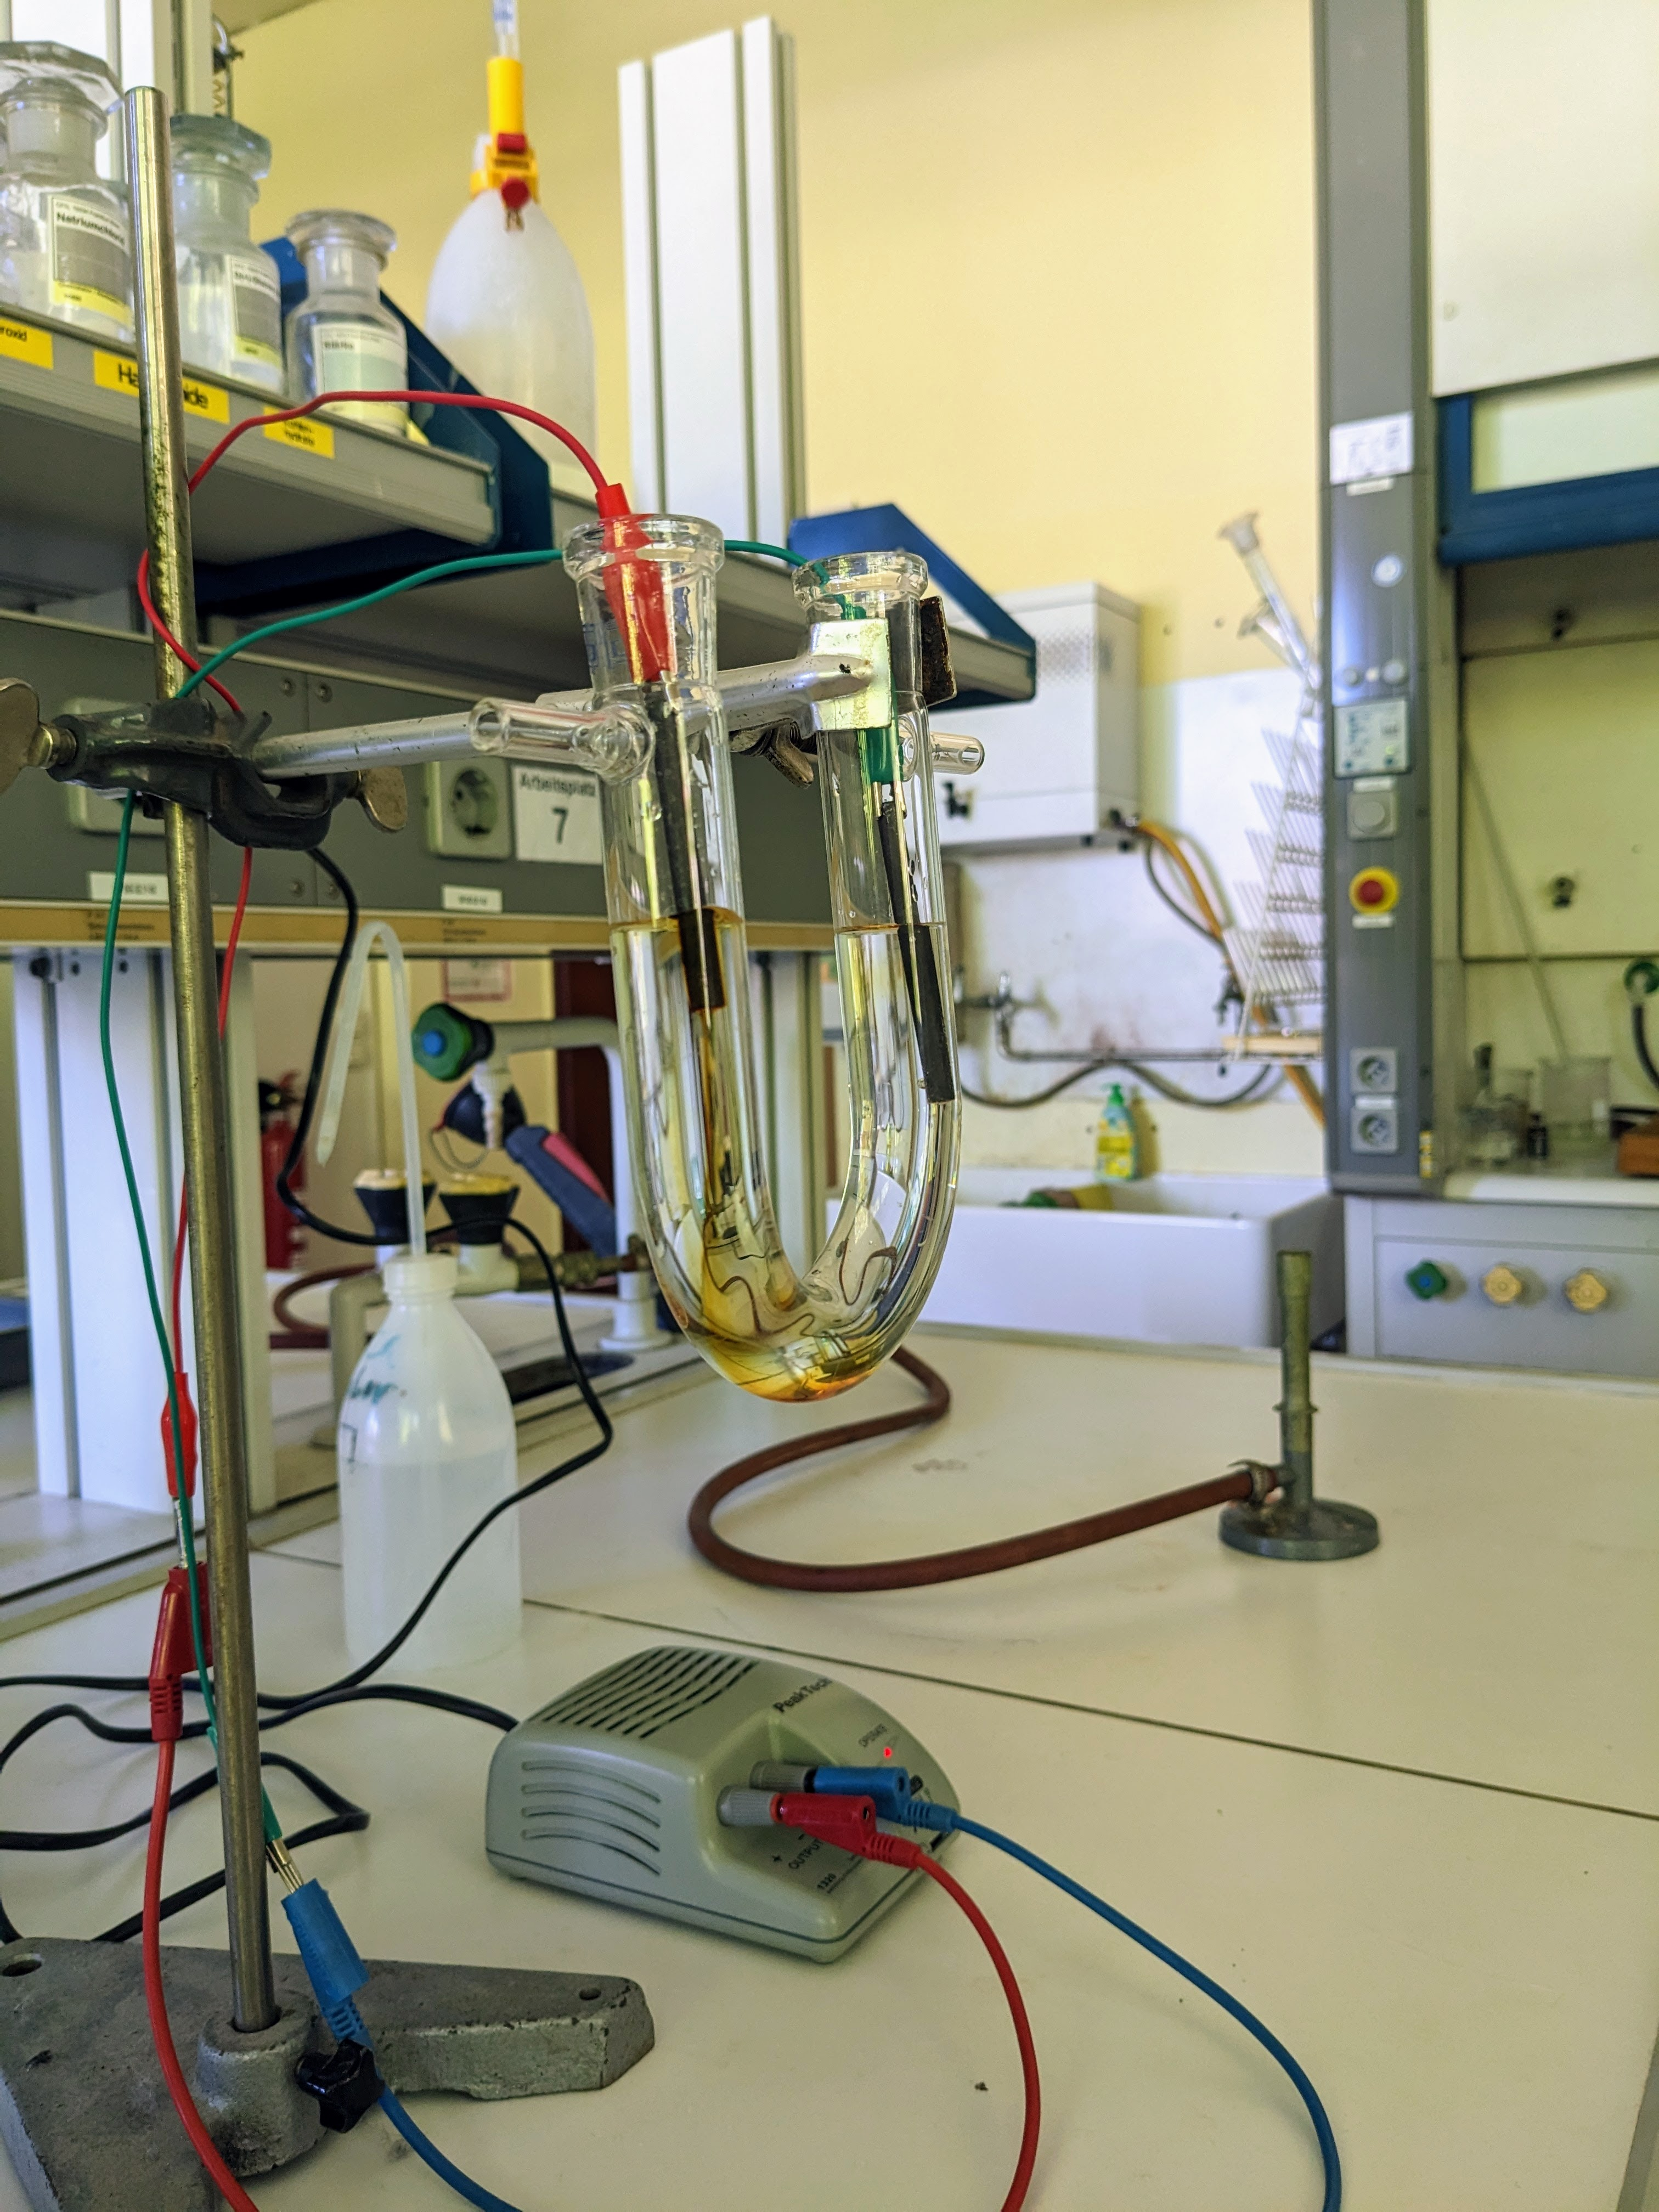
\includegraphics[scale=0.06]{beobachtung.jpg}
\end{figure}


\section{Auswertung}
Wie erwartet hat sich die farblose Kaliumiodid-Lösung nach Anschluss einer Spannung über die Stromquelle gelblich verfärbt. Wie in Abbildung \ref{fig:beobachtung} auf Seite \pageref{fig:beobachtung} zu sehen ist hängt eine Art gelber Faden an der linken Elektrode. Hier reagieren die Iodid-Ionen aus der Kaliumiodid-Lösung zu Iod, was die gelbe Verfärbung verursacht. Da das Iod oxidiert wird kann davon ausgegangen werden, dass die linke Elektrode die Anode ist, da hier eine Oxidationsreaktion abläuft. Dementsprechend findet an der anderen Elektrode, der Kathode, eine Reduktionsreaktion statt. Hier werden Kalium-Ionen zu Kalium reduziert.
\begin{center}
    \begin{equation}
        2\,I^{-} \rightleftharpoons I_{2}\,+\,2\,e^{-}
    \end{equation}
    \begin{equation}
        K^{+}\,+\,e^{-}\,\rightleftharpoons\,K
    \end{equation}
    \begin{equation}
        2\,K^{+}\,+\,2\,I^{-}\,\rightleftharpoons\,2\,K\,+\,I_{2}
    \end{equation}
\end{center}

\noindent
Bei der Entladung des Akkumulators läuft die Reaktion theoretisch in die andere Richtung ab, da es sich hierbei um eine reversible Reaktion handelt. Es findet also bei der Entladung eine Elektrolyse statt, was theoretisch zu einer Entfärbung der Lösung führen sollte. Dies konnte allerdings experimentell nicht bestätigt werden, wobei dies vermutlich auf die "übrig" gebliebene Spannung zurückführbar ist. Wie in den Daten in  Tabelle \ref{tab:messwerte} erkennbar ist steigen die Anfangswerte der gemessenen Spannungen mit jedem Versuch, was darauf hinweist, dass der Akkumulator nach 510 Sekunden noch nicht vollständig entladen war. Es wurde nicht länger gewartet, da der Verlauf der Entladekurve, wie erwartet, invers exponentiell verläuft, was zu einer sehr langen Wartezeit geführt hätte. Die Daten können in einem Spannungs-Zeit-Diagramm, Abbildung \ref{fig:absolute} visualisiert werden, wobei zugleich auch die relative Änderung der Spannung in einem Diagramm, Abbildung \ref{fig:relative} dargestellt werden kann. Die Diagramme bestätigten die Hypothese, da sie einem inversen exponentiellen Verlauf folgen, wobei offensichtlich ist, dass die verschiedenen Startwerte einen Einfluss auf die Verläufe der Diagramme haben. Zur Berechnung der relativen Werte wurde diese Formel verwendet:
\begin{center}
    \begin{equation}
        r = \frac{U_{i+1}\,-\,U_{i}}{t_{i+1}\,-\,t_{i}}
    \end{equation}
\end{center}
Hierbei ist i eine natürliche Zahl, die den Index des Datenpunktes in der Tabelle, welche sich im Anhang befindet, beschreibt und die Formel wird für jeden Wert verwendet.

\begin{figure}[h!]
    \caption{Absolute Spannungswerte gegen Zeit}
    \label{fig:absolute}
    \centering
    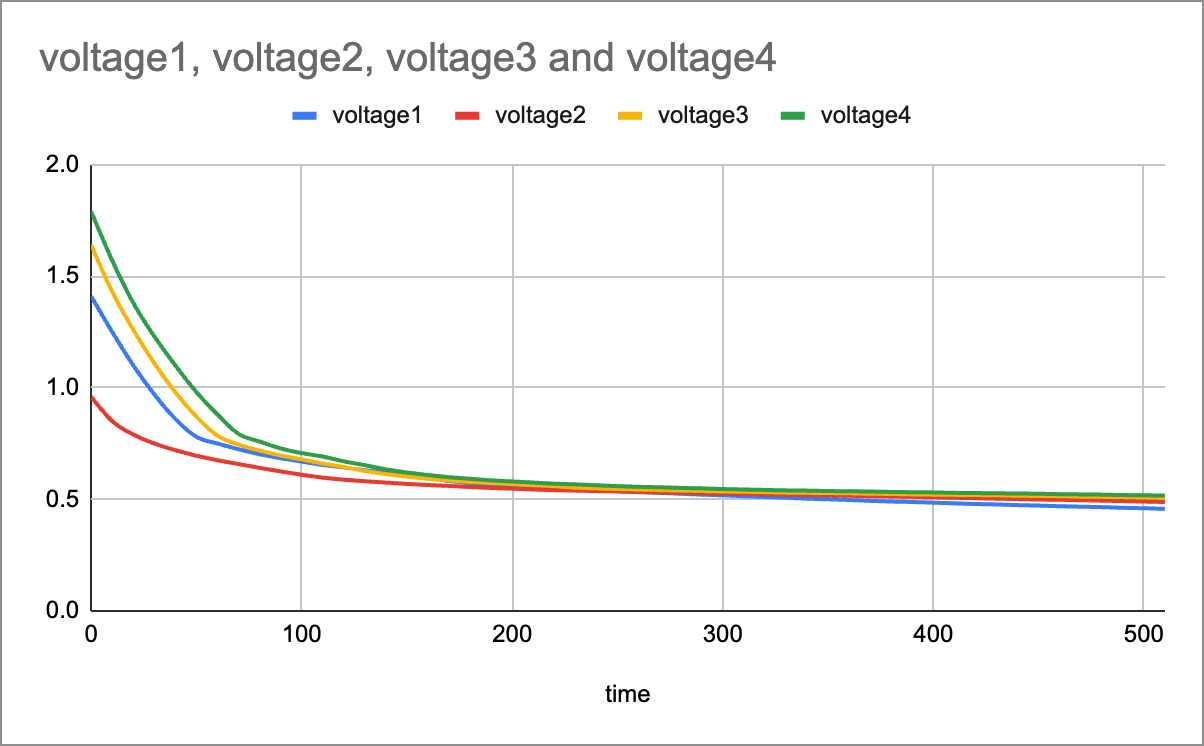
\includegraphics[scale=0.25]{absolute.png}
\end{figure}

\begin{figure}[h!]
    \caption{Relative Änderung der Spannung gegen Zeit}
    \label{fig:relative}
    \centering
    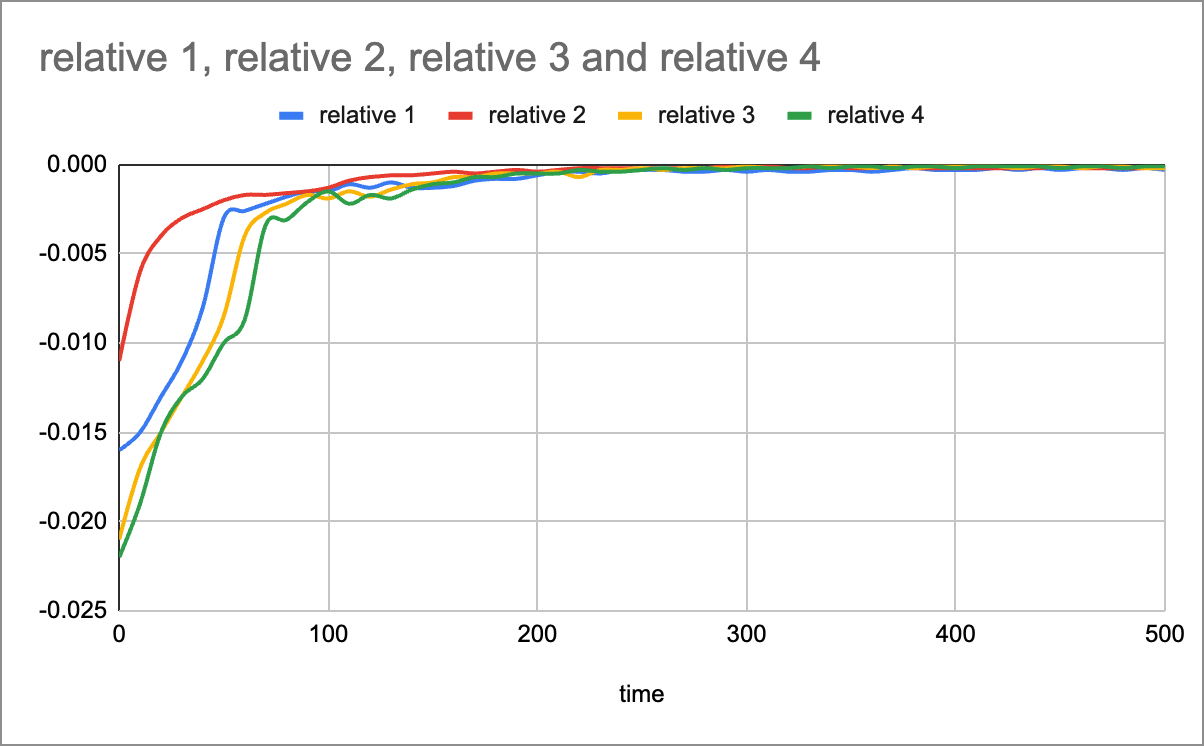
\includegraphics[scale=0.25]{relative.png}
\end{figure}
\newpage
\noindent
Um der Verfälschung der Werte durch verschiedene Startwerte entgegenzuwirken, ist es denkbar die Graphen zu dem Startwert der Kurve mit der geringsten Anfangsspannung zu verschieben. Eine solche Verschiebung liefert die Abbildungen \ref{fig:absolute_alt} und \ref{fig:relative_alt} auf Seite \pageref{fig:absolute_alt}.

\begin{figure}[h!]
    \caption{Absolute Spannungswerte gegen Zeit}
    \label{fig:absolute_alt}
    \centering
    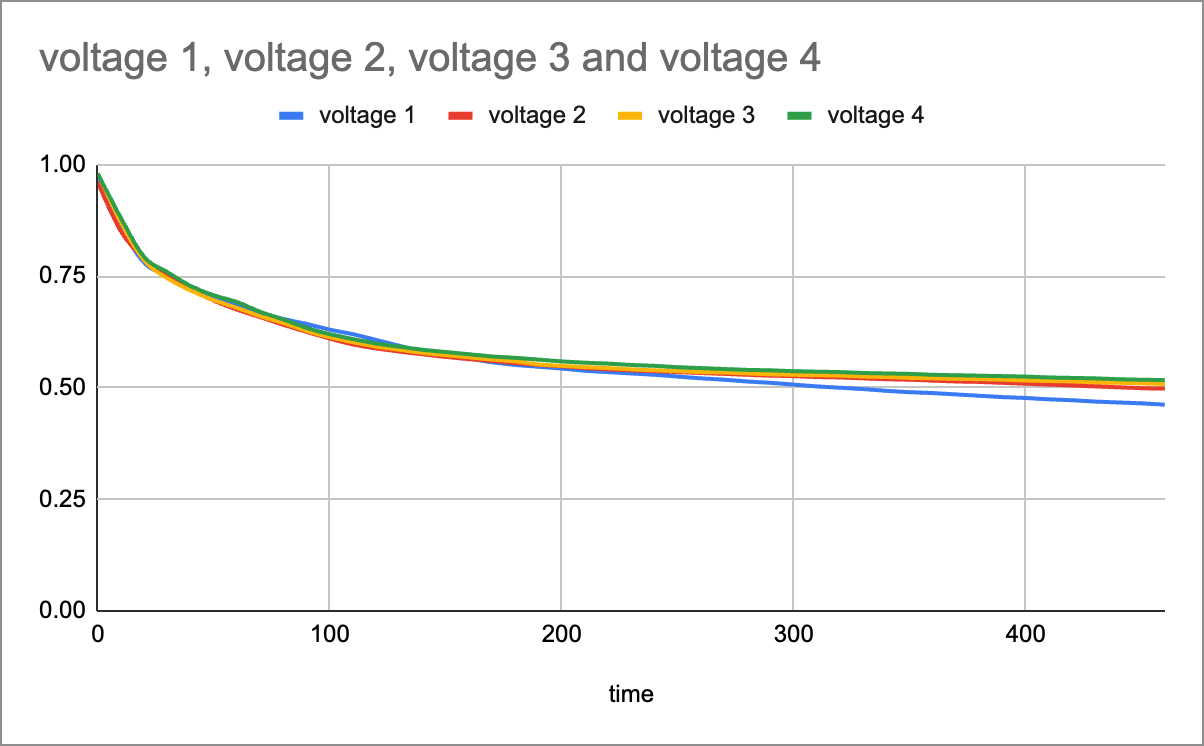
\includegraphics[scale=0.25]{absolute_alt.png}
\end{figure}

\begin{figure}[h!]
    \caption{Relative Änderung der Spannung gegen Zeit}
    \label{fig:relative_alt}
    \centering
    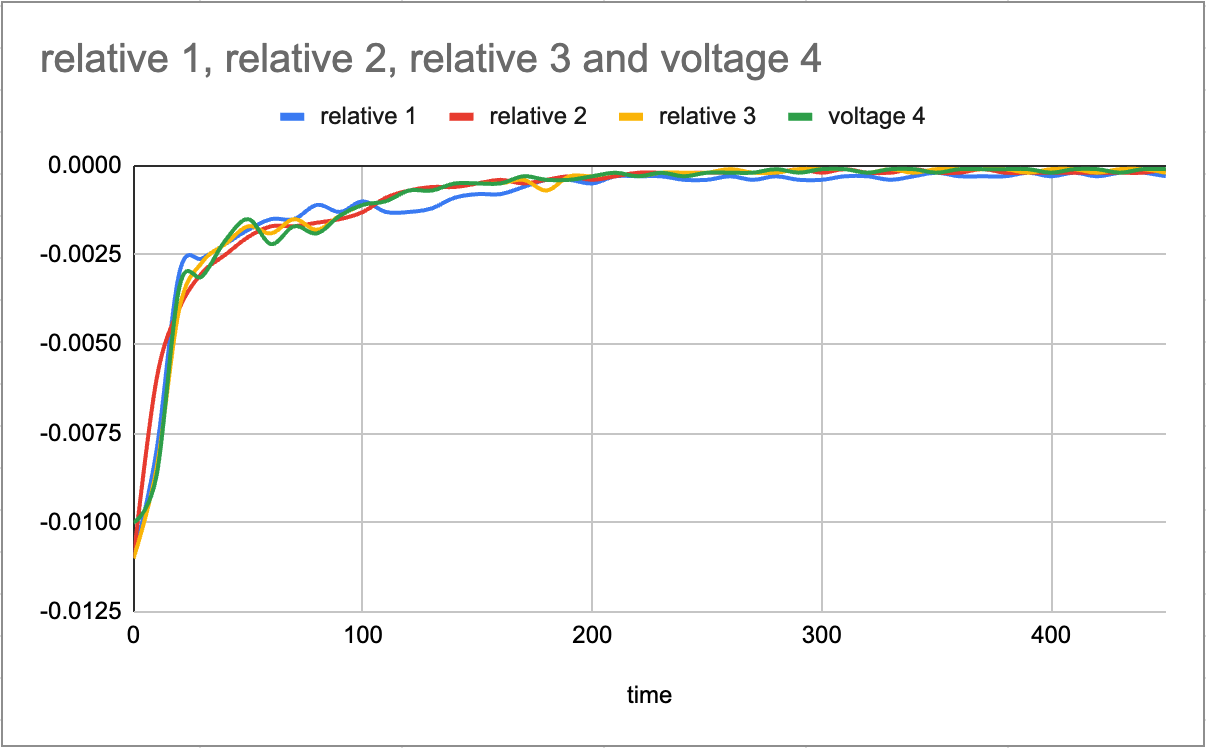
\includegraphics[scale=0.25]{relative_alt.png}
\end{figure}

\newpage
\noindent
Die vorliegenden Graphiken zeigen, dass die Entladung des Kalium-Iod-Akkumulators über mehrere Versuche, entgegen der zuvor aufgestellten Vermutung, sehr ähnlich verläuft und somit auch die Effizienz vergleichsweise konstant bleibt. Trotzdessen war der Versuch einen Kalium-Iod-Akkumulator zu bauen erfolgreich, was mit Hilfe der Entladungskurven und der Färbung der Lösung gezeigt wird.
\newpage
\section{Fehlerbetrachtung}
Zu systematischen Fehlern gehören der Fehler der Waage, der Fehler des Maßkolbens und der Fehler des Multimeters. Bis auf das Multimeter können diese Fehler allerdings vernachlässigt werden, da keine direkte quantiative Analyse durchgeführt wurde. Es wurden nur relative Werte verglichen, was bedeutet, dass auch der Fehler des Multimeters, sofern dieser konstant ist, vernachlässigt werden kann. Ein größeres Problem stellen die Messreihen dar. Zum einen wurde möglicherweise nicht immer genau nach 10 Sekunden ein Wert aufgenommen, wobei des Weiteren schlicht weg zu wenige Messreihen durchgeführt wurden. Dies ist mit der zur Verfügung stehenden Zeit begründbar. Außerdem stellt die Summierung der Spannung nach jedem Aufladen durch das Unvollständige Entladen ein Problem dar, welches allerdings durch Verschiebung der Werte umgangen werden kann. Trotzdessen ist eine solche Summierung der Spannungen nicht optimal für die Messung der Entladungskurve. Qualitativ verläuft die Entladungskurve wie erwartet, nur quantitativ ist der Abfall in der Effizienz nicht erkennbar.

\section{Quellen}
\url{https://www.chemieunterricht.de/dc2/echemie/znbr2akt.htm}\\
\url{https://www.chemieunterricht.de/dc2/echemie/vzni2akv.htm}\\
\url{https://www.chem-page.de/chemikaliendatenbank/k/kaliumiodid.html}\\
\url{https://www.seilnacht.com/Chemie/ch_zni.htm}\\
\url{https://www.tugraz.at/fileadmin/user_upload/Institute/ICTM/education/downloads/Skript_Lithium-Ionen-Batterien.pdf}\\
\url{http://u-helmich.de/che/Q1/inhaltsfeld-3-ec/3-Spannungsreihe/indexEC-3.html}\\
\url{https://www.spektrum.de/lexikon/chemie/elektronegativitaet/2841}\\
\url{https://home.uni-leipzig.de/energy/energie-grundlagen/10.html }


\newpage
\begin{table}[!htp]\centering
    \caption{Messwerte und berechnete Relative Änderung}\label{tab:messwerte}
    \scriptsize
    \begin{tabular}{l|r|r|r|r|r|r|r|r|r}\toprule
    time &voltage1 &voltage2 &voltage3 &voltage4 &relative 1 &relative 2 &relative 3 &relative 4 \\\cmidrule{1-9}
    0 &1.41 &0.96 &1.64 &1.79 &-0.0159 &-0.011 &-0.0209 &-0.022 \\
    10 &1.25 &0.85 &1.43 &1.57 &-0.0149 &-0.0059 &-0.0169 &-0.019 \\
    20 &1.1 &0.79 &1.26 &1.38 &-0.013 &-0.004 &-0.0149 &-0.0149 \\
    30 &0.97 &0.75 &1.11 &1.23 &-0.011 &-0.003 &-0.013 &-0.0129 \\
    40 &0.86 &0.72 &0.98 &1.1 &-0.0079 &-0.0025 &-0.011 &-0.012 \\
    50 &0.78 &0.695 &0.87 &0.98 &-0.003 &-0.0019 &-0.00849 &-0.009 \\
    60 &0.75 &0.675 &0.785 &0.88 &-0.002 &-0.0017 &-0.004 &-0.00869 \\
    70 &0.724 &0.658 &0.745 &0.793 &-0.0022 &-0.0017 &-0.0027 &-0.0034 \\
    80 &0.702 &0.641 &0.718 &0.759 &-0.00179 &-0.0016 &-0.0022 &-0.0031 \\
    90 &0.684 &0.625 &0.696 &0.728 &-0.0015 &-0.0015 &-0.00169 &-0.0021 \\
    100 &0.669 &0.61 &0.679 &0.707 &-0.0015 &-0.0013 &-0.0019 &-0.0015 \\
    110 &0.654 &0.597 &0.66 &0.692 &-0.0011 &-0.0009 &-0.0015 &-0.00219 \\
    120 &0.643 &0.588 &0.645 &0.67 &-0.0013 &-0.0007 &-0.0018 &-0.0017 \\
    130 &0.63 &0.581 &0.627 &0.653 &-0.001 &-0.0006 &-0.0014 &-0.0019 \\
    140 &0.62 &0.575 &0.613 &0.634 &-0.0013 &-0.0006 &-0.0011 &-0.0014 \\
    150 &0.607 &0.569 &0.602 &0.62 &-0.0013 &-0.0005 &-0.001 &-0.0011 \\
    160 &0.594 &0.564 &0.592 &0.609 &-0.0012 &-0.00039 &-0.0007 &-0.001 \\
    170 &0.582 &0.56 &0.585 &0.599 &-0.0009 &-0.0005 &-0.0007 &-0.0007 \\
    180 &0.573 &0.555 &0.578 &0.592 &-0.0008 &-0.0004 &-0.0005 &-0.0007 \\
    190 &0.565 &0.551 &0.573 &0.585 &-0.00079 &-0.0003 &-0.0005 &-0.0005 \\
    200 &0.557 &0.548 &0.568 &0.58 &-0.0006 &-0.0004 &-0.0005 &-0.0005 \\
    210 &0.551 &0.544 &0.563 &0.575 &-0.0004 &-0.0003 &-0.00039 &-0.0005 \\
    220 &0.547 &0.541 &0.559 &0.57 &-0.0004 &-0.0002 &-0.0007 &-0.0003 \\
    230 &0.543 &0.539 &0.552 &0.567 &-0.0005 &-0.0002 &-0.0003 &-0.0004 \\
    240 &0.538 &0.537 &0.549 &0.563 &-0.0003 &-0.0002 &-0.0003 &-0.00039 \\
    250 &0.535 &0.535 &0.546 &0.559 &-0.0003 &-0.0002 &-0.0002 &-0.0003 \\
    260 &0.532 &0.533 &0.544 &0.556 &-0.0003 &-0.0002 &-0.0003 &-0.0002 \\
    270 &0.529 &0.531 &0.541 &0.554 &-0.0004 &-0.0002 &-0.0002 &-0.0003 \\
    280 &0.525 &0.529 &0.539 &0.551 &-0.0004 &-0.0002 &-0.0002 &-0.0002 \\
    290 &0.521 &0.527 &0.537 &0.549 &-0.0003 &-0.0001 &-0.0002 &-0.0003 \\
    300 &0.518 &0.526 &0.535 &0.546 &-0.0004 &-0.0002 &-0.0001 &-0.0002 \\
    310 &0.514 &0.524 &0.534 &0.544 &-0.0003 &-0.0001 &-0.0002 &-0.0002 \\
    320 &0.511 &0.523 &0.532 &0.542 &-0.0004 &-0.0002 &-0.0002 &-0.0002 \\
    330 &0.507 &0.521 &0.53 &0.54 &-0.0004 &-0.0002 &-0.0001 &-0.0001 \\
    340 &0.503 &0.519 &0.529 &0.539 &-0.0003 &-0.0001 &-0.0001 &-0.0002 \\
    350 &0.5 &0.518 &0.528 &0.537 &-0.0003 &-0.0002 &-0.0001 &-0.0001 \\
    360 &0.497 &0.516 &0.527 &0.536 &-0.0004 &-0.0002 &-0.0002 &-0.0001 \\
    370 &0.493 &0.514 &0.525 &0.535 &-0.0003 &-0.0001 &-0.0001 &-0.0002 \\
    380 &0.49 &0.513 &0.524 &0.533 &-0.0002 &-0.0002 &-0.0002 &-0.0001 \\
    390 &0.488 &0.511 &0.522 &0.532 &-0.0003 &-0.0002 &-0.0001 &-0.0001 \\
    400 &0.485 &0.509 &0.521 &0.531 &-0.0003 &-0.0002 &-0.0001 &-0.0002 \\
    410 &0.482 &0.507 &0.52 &0.529 &-0.0003 &-0.0002 &-0.0001 &-0.0001 \\
    420 &0.479 &0.505 &0.519 &0.528 &-0.0002 &-0.0002 &-0.0001 &-0.0001 \\
    430 &0.477 &0.503 &0.518 &0.527 &-0.0003 &-0.0002 &-0.0002 &-0.0001 \\
    440 &0.474 &0.501 &0.516 &0.526 &-0.0002 &-0.0002 &-0.0001 &-0.0001 \\
    450 &0.472 &0.499 &0.515 &0.525 &-0.0003 &-0.0001 &-0.0001 &-0.0002 \\
    460 &0.469 &0.498 &0.514 &0.523 &-0.00019 &-0.0002 &-0.0002 &-0.0001 \\
    470 &0.467 &0.496 &0.512 &0.522 &-0.0002 &-0.0002 &-0.0001 &-0.0001 \\
    480 &0.465 &0.494 &0.511 &0.521 &-0.0003 &-0.0002 &-0.0001 &-0.0002 \\
    490 &0.462 &0.492 &0.51 &0.519 &-0.0002 &-0.0002 &-0.0002 &-0.0001 \\
    500 &0.46 &0.49 &0.508 &0.518 &-0.0003 &-0.0002 &-0.0002 &-0.0001 \\
    510 &0.457 &0.488 &0.506 &0.517 & & & & \\

    \end{tabular}
    \end{table}

\end{document}